\documentclass[11pt]{article}				% autres choix : book, report

\usepackage[utf8]{inputenc}					% gestion des accents (source)
\usepackage[T1]{fontenc}					% gestion des accents (PDF)
\usepackage[french]{babel}				    % gestion du français
\frenchbsetup{StandardLists=true}
\usepackage{textcomp}						% caractères additionnels
\usepackage{mathtools,amssymb,amsthm}
%\usepackage{mathabx}		% packages de l'AMS + mathtools
%\usepackage{lmodern}						% police de caractère
\usepackage{stmaryrd}						% symboles supplémentaires
\usepackage{csquotes}
\usepackage{empheq}							% pour encadrer.

\usepackage{biblatex}
\addbibresource{exemple.bib}

\usepackage{geometry}						% gestion des marges
\geometry{top=1.5cm, bottom=2cm, left=2.5cm, right=2.5cm}

\usepackage{booktabs}
\usepackage{graphicx}						% gestion des images
\usepackage{xcolor}							% gestion des couleurs
\usepackage{array}							% gestion améliorée des tableaux
\usepackage{multirow}
\usepackage{multicol}						% gestion améliorée des colonnes
\usepackage{subfig}
\usepackage{listings}
\definecolor{codegreen}{rgb}{0,0.6,0}
\definecolor{codegray}{rgb}{0.5,0.5,0.5}
\definecolor{codepurple}{rgb}{0.58,0,0.82}
\definecolor{backcolour}{rgb}{0.95,0.95,0.92}

\lstdefinestyle{mystyle}{
	backgroundcolor=\color{backcolour},   
	commentstyle=\color{codegreen},
	keywordstyle=\color{magenta},
	numberstyle=\tiny\color{codegray},
	stringstyle=\color{codepurple},
	basicstyle=\ttfamily\footnotesize,
	breakatwhitespace=false,         
	breaklines=true,                 
	captionpos=b,                    
	keepspaces=true,                 
	numbers=left,                    
	numbersep=5pt,                  
	showspaces=false,                
	showstringspaces=false,
	showtabs=false,                  
	tabsize=2
}

%\lstset{style=mystyle}

\usepackage[framemethod=tikz]{mdframed}		% mise en page
\usepackage{calc}							% syntaxe naturelle pour les calculs
\usepackage[pagestyles]{titlesec}			% pour les sections
\usepackage{titletoc}						% pour la table des matières
\usepackage{fancyhdr}						% pour les en-têtes
\usepackage{wrapfig}

\usepackage{tikz}
\tikzset{code/.style={draw=green!50!black, rounded corners,fill=green!5!, font=\small, text width = 0.8\textwidth}}


\usepackage{pgfplots}						% tracer des courbes
\usepackage{pgfplotstable}

\usepackage{hyperref}						% permet de mettre des url cliquables
\hypersetup{  colorlinks, citecolor = {green!40!black},  urlcolor  = {blue!60!black}}
\usepackage{listings}						% permet de mettre du code

%\usetkzobj{all}
\usetikzlibrary{calc}
\pgfplotsset{compat=1.7}

\newcommand{\tb}{\textbackslash}
\newcommand{\cmdo}[3][]{\texttt{\textbackslash #2}\texttt{[#1}\texttt{]\{#3\}}}
\newcommand{\cmdoi}[3][]{\texttt{\textbackslash #2}\texttt{[}\textit{#1}\texttt{]\{}\textit{#3}\texttt{\}}}
\newcommand{\cmd}[2]{\texttt{\textbackslash #1}\texttt{\{#2\}}}
\newcommand{\cmdi}[2]{\texttt{\textbackslash #1}\texttt{\{}\textit{#2}\texttt{\}}}


\title{\textbf{Guide d'utilisation de \LaTeX} (version Lite)
\author{Le KI'022}
\date{}
}

%\pagestyle{fancy}
%\fancyhead[L]{\textbf{Guide d'utilisation de \LaTeX}}
%\fancyhead[R]{Version Lite}
%\fancyfoot[C]{}
%\fancyfoot[R]{\thepage}
\setlength{\parindent}{0pt}
\begin{document}
\maketitle

\begin{figure}[h]
\begin{center}

\includegraphics[scale=0.5]{ressources/KI.png}
\end{center}
\end{figure}

\section*{Préambule}

Ce document a pour but de présenter les fonctionnalités de base et les plus utiles de LaTeX, ce langage étant devenu la norme pour produire des documents scientifiques aujourd'hui. Si vous ne connaissez absolument rien à ce langage pas de panique ! Ce guide est fait pour vous, il vous donnera les bases qui vous permettront d'écrire tous vos rapports et autres pendant vos années aux Ponts et Chaussées. \\

Mais d'abord je vais essayer de répondre à la question "A quoi sert {\LaTeX} ?" où plutôt: "Pourquoi me donner du mal à apprendre un langage compliqué si je peux faire plus ou moins la même chose avec Word ?". Le premier truc qu'on vous dira, c'est que LaTeX permet de faire des jolies maths, et c'est probablement ce qui vous servira le plus mais il y a d'autres manières de répondre à cette question:
\begin{itemize}
	\item LaTeX vous permet de vous concentrer uniquement sur le \textbf{contenu} de votre document et non sur la forme qui est gérée automatiquement.
	\item LaTeX demande un certain temps d'adaptation, surtout si vous êtes habitués à Word mais les documents produits sont de plus grande qualité et font plus "scientifique".
	\item Sans parler des maths, LaTeX procure une grande facilité pour ce qui est de référencer ses figures, ses graphiques, faire une bibliographie ou une table des matières. Il sera plus facile et surtout plus rapide de produire un rapport scientifique avec LaTeX car tout ce que j'ai cité se fera (presque) tout seul.
\end{itemize}  

Bonne lecture !
    
\clearpage


\section*{Commencer {\LaTeX} rapidement}

\subsection*{L'installation}

Avant d'écrire un document LaTeX, il vous faut une distribution de LaTeX. Le plus simple, rapide et efficace est d'utiliser le site \textit{Overleaf}. Il suffit de se connecter et de créer un nouveau document et\dots \ c'est tout. Il n'y a pas plus simple, le seul désavantage \footnote{Il y en a d'autres, mais peu conséquents par rapport à la facilité d'utilisation procurée par Overleaf} étant que vous allez avoir besoin d'une connexion Internet, ce qui sera rarement un soucis.\\
Pour commencer un nouveau document il vous suffit de cliquer sur "Nouveau projet" $\longrightarrow$ "Projet vide" et vous devriez tomber sur quelque chose qui ressemble à l'image ci-dessous.\\
\begin{figure}[h!]
	\centering
	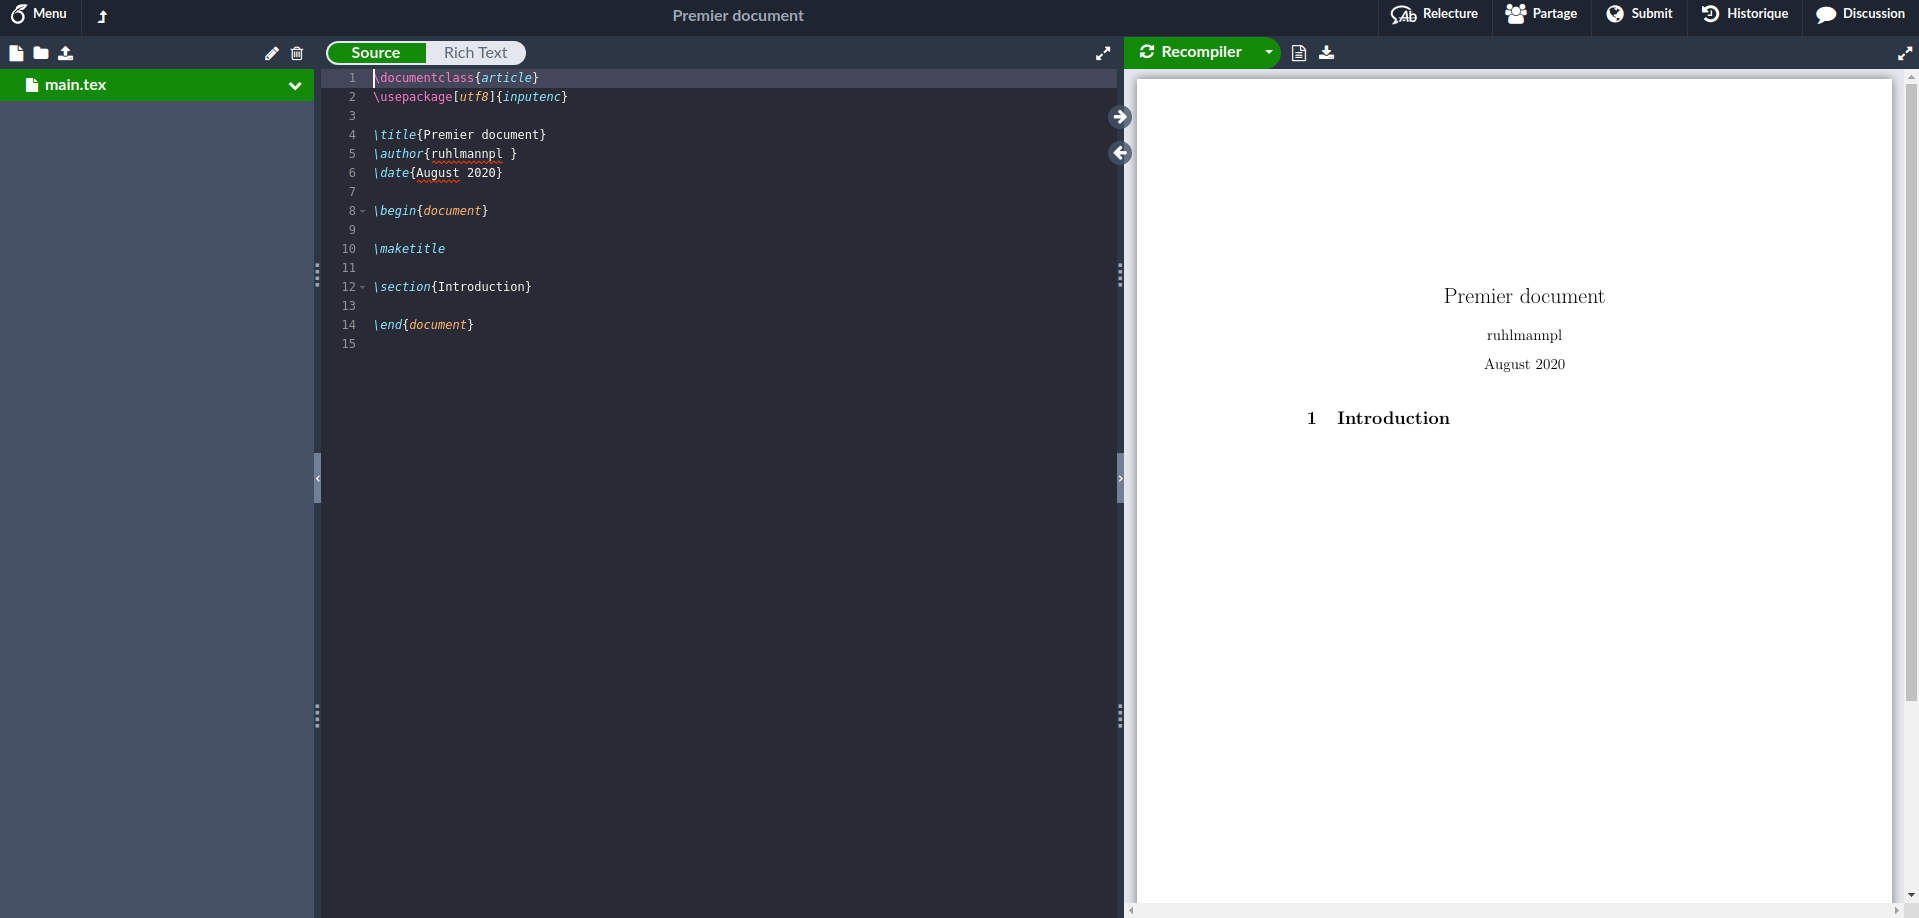
\includegraphics[scale=0.25]{ressources/overleaf_projet_vide.png}
\end{figure}	
\newline

Pour le moment, effacez tout le contenu de la page de gauche, nous  allons repartir de zéro pour cette fois. Appuyez ensuite sur le bouton "Recompiler" et vous devriez avoir une page blanche sur la droite.
Voila une des principales caractéristiques de LaTeX, contrairement à Word ou d'autres logiciels de traitements de texte, ce n'est pas du temps réel. C'est à dire que vous allez écrire du code et ensuite compiler ce code pour obtenir un document PDF. 

Je vous conseille de souvent compiler votre code pour vous rendre compte de ce que vous écrivez, vous pouvez le faire soit en appuyant sur le bouton "Recompiler" ou avec les touches Ctrl+Enter.\\



Un autre avantage d'Overleaf est qu'il vous permettra de travailler en collaboration sur un même document, chose impossible sur un éditeur classique.
Vous trouverez dans le guide complet des explications pour ceux qui voudraient avoir une distribution de LaTeX sur leur PC (Mac Linux et Windows).

\newpage

\subsection*{Les bases d'un document \LaTeX}


\noindent Pour débuter un document \LaTeX \ il faut utiliser un certain nombre de commandes et inclure des paquets\footnote{Le template fourni lors de la formation regroupe les paquets les plus utilisés en pratique.}. Voici ce à quoi chacun de vos documents devrait ressembler (commandes obligatoires en \textcolor{red}{rouge} et obligatoires pour un document en français en \textcolor{blue}{bleu}) : \\

\noindent
\textcolor{red}{\cmdoi[options]{documentclass}{type}} \\
\textcolor{red}{\cmdo[utf8]{usepackage}{inputenc}} \\
\textcolor{blue}{\cmdo[french]{usepackage}{babel}} \\
\textcolor{blue}{\cmdo[T1]{usepackage}{fontenc}} \\
~\\
\cmdoi[options]{usepackage}{nom} \\
~\\ 
\cmdi{title}{titre} \\
\cmdi{author}{auteur} \\
\cmdi{date}{date} \\
~\\ 
\textcolor{red}{\cmd{begin}{document}}\\
\texttt{\tb maketitle} \\
\texttt{\tb tableofcontents} \\
~\\
\cmdi{section}{titre de la section} \quad (\texttt{\tb section*} pour éviter la numérotation)	 \\
\cmdi{subsection}{titre de la sous-section} \\
\textit{Votre texte}\\

\cmdi{subsection}{titre de la sous-section} \\
\textit{Votre texte} \\
~\\
\textcolor{red}{\texttt{\tb end\{document\}}} \\

Vous pouvez déjà essayer de reproduire ce schéma (sans le \texttt{\tb usepackage} en noir pour le moment) avec \texttt{\tb documentclass[11pt]\{article\}}, remplacez juste ce qui est en italique par le titre, auteur, date\dots, appuyez sur Ctrl+Enter et vous devriez avoir un document qui ressemble à ceci:
\begin{figure}[h!]
\begin{center}
	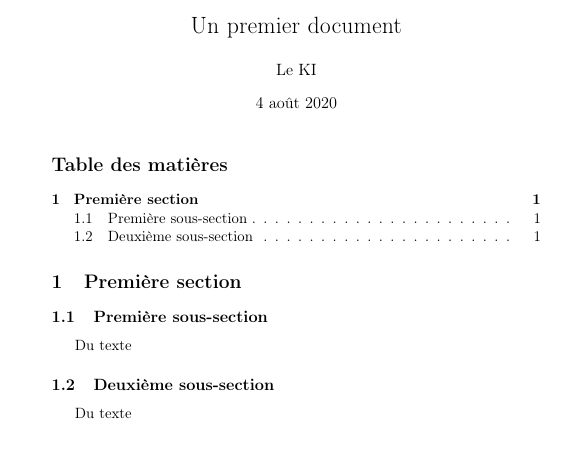
\includegraphics[scale=0.4]{ressources/frover.png}
\end{center}	

\end{figure}


Pas mal non ? En quelques lignes vous avez déjà un document prêt à être rendu.\\

$\rightarrow$ Vous avez d'autre commandes pour faire des sections, comme \texttt{\tb part  \tb chapter  \tb subsubsection} mais certaines sont spécifiques à certaines classes (ici on utilise la classe article, voir le guide complet pour en savoir plus sur les classes).

\subsection*{Les commandes classiques de mise en page}


\noindent Pour modifier le texte, il y a les commandes : \\
\begin{multicols}{2}


\begin{tabular}{lclc}
Commande &  & Rendu & Raccourci \\
\verb?\textbf{?\emph{texte}\verb?}? & $\rightarrow$ & \textbf{texte} & Ctrl + B \\
\verb?\textit{?\emph{texte}\verb?}? & $\rightarrow$ & \textit{texte} & Ctrl + I \\
\verb?\texttt{?\emph{texte}\verb?}? & $\rightarrow$ & \texttt{texte} & \\
\verb?\underline{?\emph{texte}\verb?}? & $\rightarrow$ & \underline{texte}  & \\
\verb?\emph{?\emph{texte}\verb?}? & $\rightarrow$ & \emph{texte} & \\
\verb?\textsc{?\emph{texte}\verb?}? & $\rightarrow$ & \textsc{texte} &  \\
\verb?\fbox{?\emph{texte}\verb?}? & $\rightarrow$ & \fbox{texte} & \\

\end{tabular}\\

\columnbreak

$\rightarrow$ Selon les éditeurs (Overleaf ou autre), il peut y avoir plusieurs raccourcis que ceux-ci, néanmoins il est toujours possible de les utiliser façon "Word", c'est à dire sélectionner le texte puis appuyer sur Ctrl+I pour le mettre en italique par exemple .

\end{multicols}

\begin{multicols}{2}


\noindent Les listes à puces (respectivement numérotées) se font avec les commandes suivantes : \\

\begin{tabular}{lcl}

\cmd{begin}{itemize} & ou & \cmd{begin}{enumerate} \\
\indent \verb?\item? \emph{texte} &  & \indent \verb?\item? \emph{texte} \\
\indent \verb?\item? \emph{texte} &  & \indent \verb?\item? \emph{texte} \\
\cmd{end}{itemize} &  & \cmd{end}{enumerate} \\

\end{tabular} \\

\columnbreak

$\rightarrow$ Pour des listes avec des $\bullet$ plutôt que des tirets, mettre la commande \texttt{\tb frenchbsetup\{StandardLists=true\}} en début de document (avant le \texttt{\tb begin\{document\}}). On peut également "empiler" plusieurs listes en cascade, elles seront indentées au fur et à mesure.
\end{multicols}

$\rightarrow$ En LaTeX, le \texttt{\tb begin\{\}} suivi d'un \texttt{\tb end\{\}} s'appelle un environnement, cela permet de formater ce que vous allez mettre entre ces deux commandes. \textcolor{red}{Faire attention à bien mettre le \texttt{\tb begin} et le \texttt{\tb end} sinon ça ne marchera pas !} \\


\begin{multicols}{2}


\noindent Les citations se font de la façon suivante : \\
\verb?\begin{quote}? \\
\emph{texte} \\
\verb?\end{quote}? \\

\noindent Et pour des citations de plusieurs lignes : \\
\verb?\begin{quotation}? \\
\emph{texte} \\
\verb?\end{quotation}? 

\columnbreak

\noindent La commande \verb?\footnote{?\emph{texte}\verb?}? crée une note en bas de page. \\


\noindent La position du texte sur la page se modifie avec les environnements \texttt{ flushleft, center,  flushright}. C'est certainement le 2e qui vous sera le plus utile: 
\begin{flushleft}
\verb?\begin{center}? \\
\emph{texte}\\
\verb?\end{center}? 
\end{flushleft}

\end{multicols}

\textbf{Pour les sauts de lignes et paragraphes :} \\

Vous l'avez peut-être remarqué mais en LaTeX, pour revenir a la ligne vous ne pouvez pas juste appuyer sur la touche \texttt{Enter}, il vous faut soit mettre un double backslash \texttt{\tb \tb} à la fin de votre ligne ou utiliser la commande \texttt{\tb newline}.

Vous pouvez aussi appuyer deux fois sur \texttt{Enter} mais cela créera un nouveau paragraphe, c'est à dire qu'il sera indenté par défaut (décalé vers la droite). Pour éviter cela il suffit de mettre \texttt{\tb noindent} en début de ligne ou, pour le faire pour tout le document, mettre la commande \texttt{\tb setlength\{\tb parindent\}\{0pt\}} en début de document (avant le \texttt{\tb begin\{document\}}).\\
Si vous voulez sauter une ligne, il faut alors mettre un \texttt{\tb \tb} à la fin de votre ligne puis laisser une ligne blanche comme pour faire un nouveau paragraphe.\\
Pareillement, les espaces ne se font pas en appuyant 40 fois sur la touche espace, il faut utiliser des commandes telles que \texttt{\tb quad} et \texttt{\tb qquad}.\\

$\rightarrow$ Je vous conseil d'utiliser le package \texttt{geometry} suivi de la commande\\ \verb|\geometry{top=1.5cm, bottom=2cm, left=2.5cm, right=2.5cm}|, cela vous permettra de gérer vos marges en faisant varier les valeurs \texttt{top, bottom, left} ou \texttt{right}.

\subsection*{Les images, tableaux et autres flottants}

Un des points les plus importants dans un document est l'inclusion d'images, leur référencement et les disposer intelligemment pour ne pas perturber la lecture. Sur ce point, il peut être très compliqué de vouloir faire exactement ce que l'on a en tête en LaTeX car contrairement aux logiciels Office, on ne peut pas déplacer l'image avec la souris.
Mais pour la plupart de vos documents, LaTeX va très bien gérer votre placement d'images.\\

Commençons par le plus basique, le \cmdoi[options]{includegraphics}{\textit{chemin d'accès à l'image}}.Disons que vous ayez une image \texttt{image.png} dans le même dossier que votre fichier .tex (sur Overleaf vous pouvez directement importer vos images avec un petit bouton en haut à gauche). Pour mettre cette image dans votre document il y a juste besoin d'écrire deux choses: \\

\begin{itemize}
	\item \cmd{usepackage}{graphicx} en début de document.
	\item \cmdo[scale=$x$]{includegraphics}{image.png} \quad (avec $x$ le facteur d'échelle entre 0 et 1) là où vous voulez insérer votre image.
\end{itemize}


Bien sur cette commande fonctionne dans les environnements cités ci-dessus, par exemple si vous voulez centrer votre image: \\


\begin{multicols}{2}
\cmd{begin}{center}\\
\cmdo[scale=$x$]{includegraphics}{image.png} \\
\cmd{end}{center}\\

\columnbreak

$\rightarrow$ D'autres paramètres sont possibles plutôt que le scale, voir le guide complet pour en savoir plus.
\end{multicols}


\textbf{Les flottants}\\

La méthode présentée ci-dessus permet de dire à LaTeX précisément où doivent être insérées vos images. Mais il peut être parfois plus judicieux de laisser LaTeX organiser vos images, pour cela on utilise des flottants (non ce n'est pas pareil que des flottants en info...). Les flottants tiennent leur nom du fait que LaTeX va les déplacer à sa convenance pour faire le meilleur document possible (selon lui, libre à vous de changer ensuite).\\



Prenons l'exemple de l'image précédente, nous allons maintenant la mettre dans un environnement supplémentaire nommé \texttt{figure}: \\

\begin{multicols}{2}
\cmd{begin}{figure}\texttt{[}h\texttt{]}\\
\texttt{\tb centering} \quad (Equivalent à un center)
\cmdo[scale=$x$]{includegraphics}{image.png} \\
\cmd{caption}{légende}\\
\cmd{end}{figure}\\
$\rightarrow$ Sans le \texttt{\tb centering}, l'image sera à gauche. 

\columnbreak

$\rightarrow$ L'argument "h" indique que l'on veut que notre image soit ici ("here"), c'est à dire là où on écrit le texte. On peut aussi mettre b ou t pour "top" et "bottom" par exemple, ainsi notre image se retrouvera en haut ou en bas de la page peut importe où l'on a écrit la commande.
\end{multicols}



\begin{figure}[h!]
\centering

\includegraphics[scale=0.2]{ressources/KI.png}
\caption{Le logo du KI}
\end{figure}




Voici une image incorporée dans un document avec les commandes ci-dessus. Il y a plein de manière de modifier la légende et l'image à votre convenance, comme l'encadrer, l'inclure dans du texte (package \texttt{wrapfig}) et d'autres. Plus de détails sont donnés dans le guide complet.\\


$\rightarrow$ Attention cependant, LaTeX peut décider de ne pas respecter votre argument entre crochet \texttt{[]} si cela conduit l'image à déborder de la page ou à trop éloigner le titre d'une section de son texte.\\

Un autre exemple de flottants : \textbf{les tableaux}, ceux-ci ont une syntaxe bien précise mais il existe certains sites comme \href{https://www.tablesgenerator.com/}{tablesgenerator} qui vous simplifie la vie, vous avez juste à rentrer vos donnés et il vous génère le code automatiquement.


\subsection*{Ecrire des mathématiques}

On aborde ici une grosse partie de ce que vous allez faire en LaTeX, au début cela va être un peu laborieux, car vous passerez votre temps à regarder la magnifique fiche mémo faite par le KI (disponible \href{http://latex.enpc.org}{ici}) avec entre autre les commandes mathématiques. Mais ces commandes sont assez naturelles et vous les mémoriserez assez vite.\\

$\Rightarrow$ Avant toute chose, assurez vous d'avoir mis \cmd{usepackage}{amsmath} en préambule.\\

Pour écrire des maths, c'est très simple, il suffit de se placer dans un environnement mathématique, obtenu avec \texttt{\tb( \tb)} ou \texttt{\tb[ \tb]}. 

\begin{multicols}{2}
Ainsi le code suivant:\\
\textsf{Le théorème de Pythagore \texttt{\tb(} $\text{x}^{\wedge}$2+ $\text{y}^{\wedge}$2 = $\text{z}^{\wedge}$2 \texttt{\tb)} a été prouvé faux pour des puissances supérieures. Cela veut dire que l'équation suivante n'a pas de solutions entières:
	 \texttt{\tb[} $\text{x}^{\wedge}$n + $\text{y}^{\wedge}$n = $\text{z}^{\wedge}$n \texttt{\tb}] }
	
	\columnbreak
	
	Devient sur le pdf:\\	
	Le théorème de Pythagore $x^2 + y^2 = z^2$ a été prouvé faux pour des puissances supérieures. Cela veut dire que l'équation suivante n'a pas de solutions entières: \[ x^n + y^n = z^n \]
	
	
	
\end{multicols}

Observez la différences entre les deux, le \texttt{\tb( \tb)} permet d'écrire des maths sur la même ligne que le texte en cours alors que \texttt{\tb[ \tb]} centre vos maths en sautant une ligne (\textbf{inline} vs \textbf{display} mode). Vous pouvez aussi utiliser le \$ plutôt que \texttt{\tb(} et \texttt{\tb)} pour un environnement inline.

Si vous voulez numéroter vos équations alors il faut utiliser l'environnement \texttt{equation}:
\begin{equation}
x^2 +y^2 = z^2
\end{equation}

Vous pouvez inclure toutes sortes de symboles dans un environnement mathématique comme des lettres grecques $\alpha \ \beta \ \gamma$, des signes logiques et quantificateurs $\forall \ \exists \bigcup \sum$ ainsi que les notations ensemblistes $\mathbb{RQSZ}, \mathcal{CBTL}$ (requiert le package \verb|amssymb|) La plupart de ces symboles sont répertoriés dans la fiche mémo distribuée lors de la formation ou disponible sur \href{http://latex.enpc.org}{ce site}.\\

\textbf{Puissance et indice}\\

Pour écrire des puissances et des indices, il faut utiliser \verb|^| et \verb|_|.

\begin{multicols}{2}
Le code suivant:\\

\verb|\[ a_1^2 + a_2^2 = a_3^2 \]| \\

En utilisant des \texttt{\{ \}} lorsque les exposants/indices ne sont pas réduits à un seul symbole:\\

\verb|\[ x^{2 \alpha} - 1 = y_{ij} + y_{ji} \]|\\

Plus compliqué:\\

\verb|\[ \sum_{i=1}^{\infty} \frac{1}{n^s} =| \\
\verb| \prod_p \frac{1}{1 - p^{-s}} \] |

\columnbreak
\centering
Devient sur le pdf:\\

$$ a_1^2 + a_2^2 = a_3^2$$\\
$$ x^{2 \alpha} - 1 = y_{ij} + y_{ji} $$\\
\[ \sum_{i=1}^{\infty} \frac{1}{n^s} = \prod_p \frac{1}{1 - p^{-s}} \]

\end{multicols}

\textbf{Parenthèses et accolades}\\

Vous aurez souvent besoin d'écrire des normes, des produits scalaires ou même d'encadrer une grosse expression entre parenthèse. LaTeX est fait pour gérer tout ca, j'ai listé ici quelques exemples:\\

\begin{tabular}{lc}
\vspace{11pt} Le code suivant: & Devient sur le pdf:\\
	
\verb|$\{x+y\}$| & $ \{x+y\} $ \\

\verb|$ \langle x+y \rangle $| & $ \langle x+y \rangle $ \\

\verb?$\| x+y \|$? & $\| x+y \|$ \\

\verb|\[ F = G \left( \frac{m_1 m_2}{r^2} \right) \]| & $ F = G \left( \frac{m_1 m_2}{r^2} \right) $ \\

\end{tabular}\\

Les commandes \verb|\left| et \verb|\right| permettent d'ajuster la taille de vos parenthèses (marche avec \verb|[] {} ...|) à l'expression entre les deux. Ces commandes sont indissociables, l'une ne peut venir sans l'autre, ainsi si vous voulez juste mettre une parenthèse à gauche il vous faudra mettre un \verb|\right.| (le point est inclus) à la fin de votre expression et un \verb|\left(| au début.\\

$\rightarrow$ Si jamais \verb|\left| et \verb|\right| ne donnent pas le résultat souhaité, vous pouvez essayer \verb|\big \Big \bigg \Bigg| (ordre de taille croissante).\\


\textbf{Espaces en mode math}\\

En mode math (c'est à dire entre \verb|$ $| ou \verb|\[ \]| ) on ne peut pas espacer les caractères, symboles ou expression en appuyant simplement sur la touche espace, LaTeX fera comme si tout fait partie d'un même mot. Pour manuellement mettre un espace dans une expression il vous faudra donc utiliser un des symboles suivants :\\

\begin{center}
	\begin{tabular}{lcr}
	
	Commande & Code   &  Rendu \\ 
	
	\verb|\!|  & \verb|$x^2\! +3x\! +2$| & $ x^2\! +3x\! +2$   \\ 
	 
	\verb| Espace |&\verb|$x^2   + 3 x+  2$|  & $x^2+3x+2$ \\ 
	 
	 \verb|\,| & \verb|$x^2\, +3x\, +2$| & $x^2\, +3x\, +2$ \\ 
	 
	 
	 \verb|\ | & \verb|$x^2\ +3x\ +2$| &  $x^2\ +3x\ +2$ \\ 
	 
	\verb|\quad | & \verb|$x^2\quad +3x\quad +2$| & $x^2\quad +3x\quad +2$  
\end{tabular}
\end{center} 

\textbf{Equations}\\

En LaTeX vous pouvez présenter vos équations de la manière suivante:

\begin{multicols}{2}

\cmd{begin}{equation} \\
\cmd{label}{eq1} \\
\verb|f(x)  = 3x(x+1) | \\
\cmd{end}{equation} 

\columnbreak

$\rightarrow$ Il faut utiliser \cmd{begin}{equation*} si vous ne voulez pas numéroter votre équation. Le \verb|\label| quant à lui permet de faire des références à l'équation par \verb|\ref{eq1}|.

\end{multicols}
Si vous voulez couper votre équation sur plusieurs lignes, il faut utiliser l'environnement \verb|split|.
\begin{multicols}{2}
\cmd{begin}{equation} \cmd{label}{eq1} \\
\cmd{begin}{split} \\
\verb|f(x) & = 3x(x+1) \\ | \\
\verb|& = 3x^2 + 3x | \\
\cmd{end}{split} \\
\cmd{end}{equation} 

\columnbreak

\begin{equation} \label{eq1}
\begin{split}
f(x) & = 3x(x+1) \\
& = 3x^2 +3x
\end{split}
\end{equation}
	
\end{multicols}

Si maintenant vous voulez aligner plusieurs lignes, soit pour plusieurs équations ou juste pour développer un calcul, l'environnement \verb|align| est parfait:

\begin{multicols}{2}

\cmd{begin}{align} \quad (Ou \verb|align*| )\\
\verb|2x - 5y &= 8 \\| \\
\verb|3x +9y &= -12| \\
\cmd{end}{align} \\

\columnbreak

$\rightarrow$ Le \verb|&| sert à aligner l'équation verticalement, on le met généralement au niveau du signe égal, à noter que vous pouvez en mettre plusieurs sur une même ligne.

\end{multicols} 
Les matrices s'écrivent d'ailleurs avec une syntaxe similaire, il faut utiliser l'environnement \texttt{pmatrix} et séparer les coefficients avec des \verb|&| et utiliser des \verb|\\| pour changer de ligne.\\  

Voilà pour le principal, il y a bien sur une multitude d'autres environnement qui permettent d'augmenter la complexité, vous trouverez dans le guide complet une présentation de ces fonctionnalités. \\
J'aimerais ici finir par quelque chose qui vous sera sûrement utile : \textbf{définir une fonction en mathématiques}.
\begin{multicols}{2}
	
\verb|\[ f: \left | \\
\verb|\begin{array}{rcl}| \\
\verb|\mathbb{R} & \longrightarrow & \mathbb{R} \\|	\\
\verb|x & \longmapsto & \begin{cases} \frac{x^2}{2} &| \\ \verb|\textrm{si } x > \geq 0 \\| \\
\verb|\frac{\pi^2 + \frac{1}{x}}{2} & \textrm{si } x < 0 | \\ 
\verb|\end{cases}| \\
\verb|\end{array} \right. \]|
	
\columnbreak	

\[
f: \left|
\begin{array}{rcl}
	\mathbb{R} & \longrightarrow & \mathbb{R} \\
	x & \longmapsto & \begin{cases} x^2/2 & \textrm{si } x \geq 0 \\
	\frac{\pi^2 + \frac{1}{x}}{2} & \textrm{si } x < 0 \end{cases}
\end{array} \right. \]
\end{multicols}

Bien sur cet exemple est un degré de complexité au dessus de ce que vous pourriez être amenés à faire, mais il vous suffit de le modifier à votre convenance.


\clearpage
\subsection*{Inclure du code}
Dans la plupart de vos TPs, vous aurez à compléter un code Python ou même juste à le faire tourner pour faire une approximation numérique, un calcul de déformations, etc. Il vous faudra donc inclure dans votre compte-rendu la partie du code la plus importante que vous avez écrite. Pour cela, LaTeX vous propose le package \texttt{listings}.

En n'oubliant pas de charger ce package en préambule de votre document, vous pourrez inclure du code de cette façon:

\begin{lstlisting}[language=Python]
import math as m
import numpy as np
import scipy as sp
import matplotlib.pyplot as plt

def OpenPtsFile(filename): #function to import data in Pts file
	f = open(filename,'r')
	print ('Reading file ' + filename)
	s = f.readline()
	vals = s.split("\t")
	npts = int(vals[0])
	nraw = int(vals[1])
	ncol = int(vals[2])
	print(npts, 'points,', nraw, 'raws,', ncol, 'columns')
	Pts = np.zeros(shape=(nraw, ncol, 2))
\end{lstlisting}

Ce résultat est celui obtenu en faisant un simple copier-coller du code source, vous pouvez d'ailleurs éviter cette démarche par la commande :\\
 \verb|\lstinputlisting[language=Python, firstline=2, lastline=23]{moncode.py}| qui va inclure votre code source de la ligne \texttt{firstline} (=2) à la ligne \texttt{lastline} (=23) puis le mettre en forme comme ci-dessus.\\

\textbf{Rendre le code plus joli :}\\

Il est possible de modifier l'aspect visuel du code dans votre document en définissant un \texttt{style} par l'intermédiaire de la commande \verb|\lstdefinestyle|. Les possibilités étant très nombreuses, je ne vais pas vous décrire toutes les options possibles, je vous montre plutôt un exemple de ce qu'il est possible de faire. Un petite recherche sur internet\footnote{Vous pouvez aussi consulter la documentation du package \texttt{listings} disponible \href{https://ctan.gutenberg.eu.org/macros/latex/contrib/listings/listings.pdf}{ici}} vous permettra d'en savoir plus.\\

\lstset{style=mystyle}
\begin{lstlisting}[language=Python]
import math as m
import numpy as np
import scipy as sp
import matplotlib.pyplot as plt

def OpenPtsFile(filename): #function to import data in Pts file
f = open(filename,'r')
print ('Reading file ' + filename)
s = f.readline()
vals = s.split("\t")
npts = int(vals[0])
nraw = int(vals[1])
ncol = int(vals[2])
print(npts, 'points,', nraw, 'raws,', ncol, 'columns')
Pts = np.zeros(shape=(nraw, ncol, 2))
\end{lstlisting}  

\clearpage
\subsection*{Faire une bibliographie}

Cette section est un peu plus technique car elle requiert l'usage d'un fichier tiers qui vous permettra de faire votre bibliographie. En premier lieu, il vous faut le package \verb|biblatex|, importez-le, puis suivez les étapes suivantes :

\begin{itemize}
	\item \underline{Étape 1 :} Sur Overleaf, cliquez sur le bouton "New File" en haut à gauche de l'écran (sous le bouton menu). Écrivez "exemple.bib" dans la zone de texte puis créez votre fichier.\\
	
	\item \underline{Étape 2 :} Ensuite dans votre fichier .tex, il faut ajouter la ligne \cmd{addbibresource}{exemple.bib} en dessous de votre \cmd{usepackage}{biblatex}.\\
	
	\item \underline{Étape 3 :} Dans votre fichier "exemple.bib", copiez-collez le texte suivant :
	\begin{flushleft}
		\verb|@book{guidelatex,| \\
		\qquad \quad	\verb|author = {Le KI'022},| \\
		\qquad	\quad \verb|title = {Guide d'utilisation de \LaTeX},| \\
		\qquad  \quad \verb|year = {2020},| \\
		\verb|}| \\
		
	\end{flushleft}
	
	\item \underline{Étape 4 :} Maintenant, il vous faut écrire un petit texte pour citer le guide, par exemple:
	
	"J'utilise le guide LaTeX du KI \cmd{cite}{guidelatex}\footnote{L'argument du \texttt{\tb cite} est le premier argument de \texttt{\tb @book\{...\}}.} pour pouvoir écrire mes rapports en première année des Ponts."
	
	Puis ajoutez simplement la commande \verb|\printbibliography| à la fin de votre document.\\
	
	\item \underline{Bonus :} Vous pouvez écrire \verb|\printbibliography[heading=bibintoc, title=Bibliographie]| pour ajouter votre bibliographie à la table des matières (nécessite le \verb|\tableofcontents|).
	
\end{itemize}
\begin{figure}[h!]
	\centering
	\subfloat[Sans la table des matières]{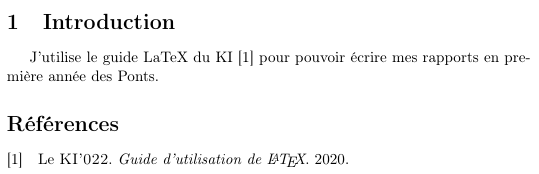
\includegraphics[width=0.5\textwidth]{ressources/testbib1.png}} \hfill
	\subfloat[Avec la table des matières]{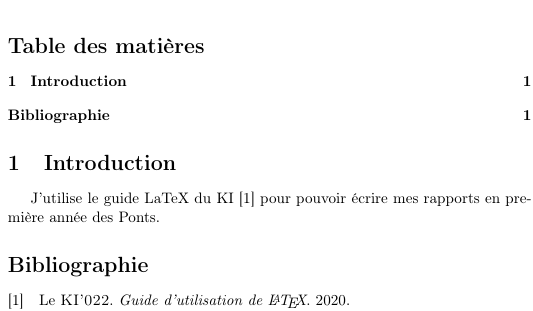
\includegraphics[width=0.5\textwidth]{ressources/testbib2.png}}

\end{figure}

$\rightarrow$ Voila la marche à suivre, en fonction des œuvres à citer, il vous faudra juste changer l'étape 3 en mettant d'autres œuvres comme des articles \verb|@article|, des thèses \verb|@thesis|,... .

\newpage

\subsection*{Créer vos propres commandes}

Cette section n'apportera rien de plus à vos documents LaTeX, elle vous fera simplement gagner du temps à l'écriture. Mais lorsque vous devrez écrire des rapports de TP en AnaCS par exemple, il vous faudra écrire beaucoup de normes, intégrales et autres expressions qui partagent beaucoup de caractéristiques communes.\\

Voyons un exemple pour illustrer mes propos:\\


\begin{multicols}{2}
	\begin{tabular}{l|c}
Code	&  PDF \\ 
\verb? $ \| u \|_{\mathcal{H}^1_0 ? &  \( \| u \|_{\mathcal{H}^1_0 \left( \Omega \right) } \)  \\
	\verb? \left( \Omega \right) $?   &  
\end{tabular}

\columnbreak

$\rightarrow$ L'idéal serait d'avoir une commande \verb|\norme{u}| qui donnerait le même rendu que le code de gauche.
\end{multicols} 

Heureusement, nous pouvons en LaTeX définir nos propres commandes de façon assez simple. Avant de s'attaquer à l'exemple ci-dessus, voyons-en un plus simple.

Par exemple, la commande \cmd{mathbb}{R} peut s'avérer redondante lorsque l'on doit faire beaucoup intervenir ce symbole ($ \mathbb{R} $).

Pour cela, il vous suffit d'écrire en préambule de votre document (avant le \cmd{begin}{document}) : 
\begin{multicols}{2}

\begin{center}
	\cmd{newcommand\{\tb R\}}{\tb mathbb\{R\}}.
\end{center}
 
\columnbreak

$\rightarrow$ Le \verb|\R| est le nom de votre commande tandis que le \cmd{mathbb}{R} est ce que votre commande va effectuer. Voilà, maintenant, pour écrire $ \mathbb{R} $ il vous suffira d'écrire \verb|\R|.\\
\end{multicols}

Maintenant il faudrait que votre commande puisse accepter des paramètres, c'est à dire de la forme \cmdi{macommande}{argument}. Il faut donc modifier la commande précédente ainsi :

\begin{multicols}{2}
	
	\begin{center}
		\cmdo[1]{newcommand\{\tb bb\}}{\tb mathbb\{\#1\}}
	\end{center}
	
	\columnbreak
	
	$\rightarrow$ Le \verb|\bb| est le nom de votre commande tandis que \verb|[1]| est le nombre d'arguments. Enfin \cmd{mathbb}{\#1} est ce que fait votre commande, le \verb|#1| sera remplacé par le texte que vous mettrez dans \verb|\bb{...}|\footnote{Si le nombre d'arguments est supérieur à 1, vous y ferez référence avec \texttt{\#1, \#2,}etc . Et pour utiliser votre commande vous devrez écrire \texttt{\tb macommande}\{\textit{argument 1}\}\{\textit{argument 2}\}...\{\textit{argument n}\}.}.
\end{multicols}

Voilà, nous pouvons maintenant écrire la commande vue au début de la section, nous voulons un seul paramètre, la fonction \texttt{u}, tout le reste doit être fixé:
\newcommand{\norme}[1]{\|#1\|_{\mathcal{H}^1_0\left(\Omega\right)}}
\begin{center}
	\cmdo[1]{newcommand\{\tb norme\}}{\tb |\#1\tb|{\_}\{\cmd{mathcal}{H}\textasciicircum 1\_0 \tb left( \tb Omega \tb right)\}} \\
\end{center}



Ainsi, si vous êtes dans un environnement math, la commande \cmd{norme}{u} vous produira $\norme{u}$.\\

\textbf{Conclusion}\\

Merci d'avoir lu ce guide, j'espère qu'il vous aura été utile et que les explications étaient assez claires. Si jamais vous voulez en savoir plus, sur n'importe quel aspect de ce qui a été présenté ici, je vous invite à consulter le guide complet disponible sur \href{http://latex.enpc.org}{ce site}. Et surtout n'oubliez pas que \textbf{Google est votre ami}, la plupart de vos questions ont déjà été posées \textbf{et} répondues sur plein de forums.\\

N'hésitez pas à me faire part de vos remarques ou commentaires, soit par mail à l'adresse \\ \texttt{pierre-louis.ruhlmann@eleves.enpc.fr} ou en contactant le KI par Facebook ou sur \href{http://clubinfo.enpc.org}{son site}.\\



\end{document}